
\section{\sysname System Overview}
\label{sec:system-overview}

To break the prefill-side storage I/O bottleneck, we propose a \textbf{dual-path loading} architecture that fundamentally rethinks how KV-Cache is retrieved in PD-disaggregated inference. Based on this architecture, we design and implement \sysname.
\sysname adopts two widely-adopted techniques demonstrated in \autoref{sec:background}:
(1) \textbf{PD Disaggregation}~\cite{OSDI24:DistServe,ISCA24:Splitwise}, which separates prompt and decode processing for better efficiency.
(2) \textbf{Layerwise prefill}, which avoids HBM bottlenecks recognized by LayerKV~\cite{LayerKV} and PrefillOnly~\cite{SOSP25:PrefillOnly} on prefill engines and improves GPU utilization.

Our system consists of the following components:
\begin{itemize}[leftmargin=*]
    \item \textbf{Inference Engines.} Each engine manages one GPU.
    Engines are categorized into prefill engines (PEs) for prefill and decoding engines (DEs) for decode.
    \item \textbf{Traffic Manager (\autoref{sec:traffic-manager}).} Each engine contains a traffic manager to conduct (1) Host-Device memory copies (H2D \& D2H), (2) KV-Cache transfers between PEs and DEs, and (3) KV-Cache reads/writes from/to storage via the storage NIC. We adopt a CNIC-centric traffic management approach, detailed in \autoref{sec:traffic-manager}, to prevent KV-Cache traffic from affecting communications in model inference.
    \item \textbf{Request Scheduler (\autoref{sec:scheduling}).} A central scheduler that receives client requests and distributes them across engines. It is also responsible for dynamically distributing data traffic between two paths (\autoref{fig:dual-path-loading}).
\end{itemize}

\begin{figure*}[t!]
  \centering
   \begin{subfigure}[b]{0.45\textwidth}
     \centering
      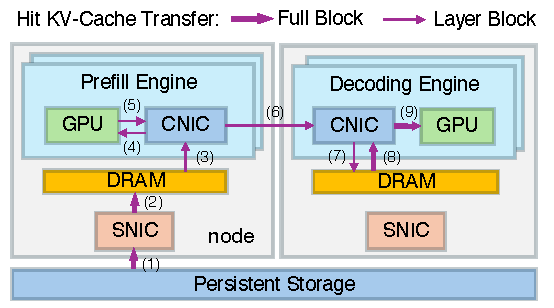
\includegraphics[width=\textwidth]{figures/dataflow_peread.pdf}
      \caption{\normalfont PE Read Path}
      \label{fig:pe_flow}
    \end{subfigure}
    \hspace{6mm}
    \begin{subfigure}[b]{0.45\textwidth}
        \centering
      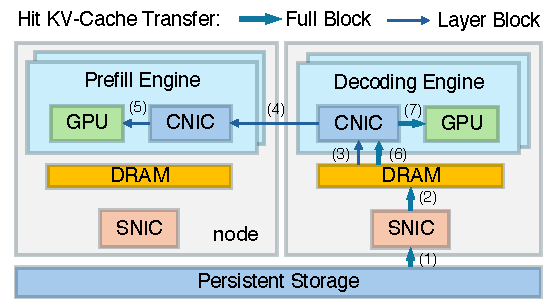
\includegraphics[width=\textwidth]{figures/dataflow_ceread.pdf}
      \caption{\normalfont DE Read Path}
      \label{fig:de_flow}  
    \end{subfigure}
    \caption{\normalfont Dual-path loading illustration. The scheduler dynamically distributes data traffic between the two paths.}
    \label{fig:dual-path-loading}
\end{figure*}


\subsection{Dual-Path Loading}
\label{sec:dual-path-loading}

In addition to the conventional \emph{storage-to-prefill} path, \sysname introduces a novel \emph{storage-to-decode} path, allowing KV-Cache to be loaded first into a decode engine and then transferred to the prefill engine via high-bandwidth RDMA over the compute network. 
By dynamically distributing load across both paths, the system aggregates the storage NIC bandwidth of all engines --- including otherwise-idle decode-side NICs --- and eliminates the asymmetric bandwidth saturation that limits existing systems. This approach transforms the storage I/O from a single-bottleneck resource into a globally pooled and schedulable capacity. % The following subsections detail the data-flow design and prove its feasibility under typical deployment ratios.
The exact data flows of the dual-path are described below.

To implement dual-path loading, \sysname allocates a small amount of DRAM as buffers on each PE and DE, called \emph{PE buffer} and \emph{DE Buffer}.
% In \autoref{fig:pe_flow} and \autoref{fig:de_flow}, we ignore all newly computed KV-Cache, since its volume is bounded by the GPU's compute capacity and is therefore relatively small.

\parabf{Prefill PE read path.}
First, the KV-Caches of hit tokens are read from persistent storage into the PE buffer (as Label 1 and 2 shown in \autoref{fig:pe_flow}). 
Before the computation of an attention layer, those KV-Caches of that layer are transferred to PE HBM (3 and 4) to compute the KV-Cache of cache-miss prompt tokens.
Then, all KV-Caches of both hit and miss tokens are transferred to the DE buffer to form the complete prompt KV-Cache (5-7). This process (3-7) repeats $n_{layer}$ times.
During the prefill forward pass, transfers overlap with computation.

\parabf{Prefill DE read path.} The KV-Caches of hit tokens are first read into DE buffer (as Label 1 and 2 shown in \autoref{fig:de_flow}).
During PE prefill, KV-Cache for the corresponding layer is read from the DE buffer, also overlapping with computation (3-5). This process repeats $n_{layer}$ times.
After a layer's computation completes, only the KV-Caches of miss tokens are transferred to DE buffer and merged with the existing hit token KV-Cache.

\parabf{Decode Phase.} After receiving the complete prompt KV-Cache in DE buffer (including loaded KV-Cache via PE read path and the KV-Cache of newly appended tokens), the decode phase begins.
The DE first allocates HBM and performs host-to-device (H2D) transfers (Label 8 and 9 in \autoref{fig:pe_flow}; Label 6 and 7 in \autoref{fig:de_flow}), then releases CPU memory before starting decode.
The design of DE buffer imposes bandwidth pressure on DRAM and CNIC (an extra H2D), which could be avoided by directly bypassing it via GPU Direct RDMA.
However, since the generation length is typically short in this scenario, time-to-first-token (TTFT) accounts for a non-negligible portion of the total end-to-end request time.
Introducing DE buffer helps reduce GPU memory usage.
During decode, whenever a full block of tokens (e.g., 64 tokens) is accumulated, it is immediately persisted to disk.

\parabf{Different Block Layouts.}
We adopt two different block layouts: \emph{Full Block} and \emph{Layer Block}, which contain all layers and a single layer, respectively.
Detailed layout can be found in \autoref{subsec:block-layout}.
For all interactions with storage, we adopt Full Blocks.
In the PE read case, KV-Cache loading to PE HBM and transfer to DE Buffer occur in a layerwise streaming fashion, both using Layer Blocks.
Similarly, for the DE read path, transfers from the DE Buffer to the PE HBM use Layer Blocks.




\subsection{Bottleneck-Free Analysis}
\label{subsec:bottle-free-analysis}
We demonstrate that the system can fully saturate all storage NICs without introducing compute-NIC or DRAM bottlenecks, under most reasonable P/D ratios.
We assume a well-configured PCIe topology (each pair of GPU--NIC is under the same PCIe switch), load-balanced task scheduling, no congestion on the computation network, and that storage read bandwidth is fully utilized.

\parabf{Notation.} Let $P$ and $D$ denote the number of prefill and decode nodes, respectively. Each node has $g$ GPUs, each with one compute NIC of bandwidth $B$. The storage bandwidth per machine is $s \times B$ (shared by all engines on that machine); $M$ is the memory bandwidth per machine.

\parabf{Traffic per PE-DE pair.} We assume that the storage read bandwidth is fully utilized and that task scheduling is load-balanced. Under load balancing, storage NIC bandwidth is evenly shared. The traffic per pair for the PE read path (all steps in \autoref{fig:pe_flow}) is $T_p = Bs/(Dg^2)$; for the DE read path (\autoref{fig:de_flow}) it is $T_c = Bs/(Pg^2)$. Link traffic is the sum over all pairs using that link.



\parabf{PE CNIC Bandwidth Analysis.}
For PE CNIC, loopback traffic (i.e., H2D and D2H that does not traverse switches) exists, so the total traffic on the PCIe side is always greater than or equal to the switch-direction traffic, regardless of read or write operations.
Therefore, we only need to compute the pressure on the PCIe side.
Read operations include PE paths (3) and (5), with total traffic over all pairs:
\begin{align}
2\times T_p \times Dg = 2Bs/g \leq B
\end{align}
Since $s\leq g$ always holds in practice, the read direction is always bottleneck-free.
Write operations include PE path (4) and DE path (5), with total traffic:
\begin{align}
(T_p + T_c) \times Dg = Bs/g \times (1 + D/P) \leq B
\end{align}
Then, we obtain:
\begin{align}
P/D \geq \frac{s}{g-s}
\end{align}

\parabf{DE CNIC Bandwidth Analysis.}
For DE CNIC, read operations include PE path 8 and DE paths 3/6, with traffic:
\begin{align}
(T_p + T_c \times 2) \times Pg = s/g\times (P/D+2) \times B \leq B
\end{align}
Then, we obtain:
\begin{align}
P/D \leq \frac{g-2s}{s}
\end{align}

Write operations include PE paths 7/9 and DE path 7, with traffic:
\begin{align}
(2T_p + T_c) \times Pg \leq B
\end{align}
This implies:
\begin{align}
P/D \leq \frac{g-s}{2s}
\end{align}

\parabf{DRAM Pressure Analysis.}
DRAM is half-duplex, so we sum the read and write pressures.
For PE MEM, the pressure is $2sB$, which generally does not exceed memory bandwidth.
For DE MEM, following the similar analysis above, we can get the pressure is $(3 + 2P/D) Bs$.
Requiring the DE MEM pressure to be less than or equal to $M$, we obtain:
\begin{align}
P/D \leq \frac{M/Bs - 3}{2}
\end{align}

\parabf{Summary.} Combining all the above analyses, we have:
\begin{align}
\frac{s}{g-s} \leq P/D \leq \min\left\{\frac{g-2s}{s}, \frac{g-s}{2s}, \frac{M/Bs - 3}{2}\right\}.
\end{align}
For $(g=8, s=1)$ with $M \approx 500$ GB/s and $Bs \approx 50$ GB/s, the bottleneck-free range is $\frac{1}{7} \leq$ P/D $\leq \frac{7}{2}$, which covers most practical configurations.


\subsection{Practical Challenges}
\label{sec:system}

The dual-path architecture fundamentally reorients data movement: KV-Cache can be loaded either directly from storage into prefill engines or indirectly via decode engines, thereby aggregating storage bandwidth across all engines and breaking the prefill-side I/O bottleneck. However, realizing this high-level design in a practical system introduces three interrelated challenges. We briefly outline these challenges below and refer the reader to the corresponding sections for details.

\parabf{Fine-grained data transfer (\autoref{sec:traffic-manager}).} 
The layer-wise execution paradigm, while essential for overcoming HBM capacity limits, fragments the KV-Cache into numerous fine-grained blocks \cite{ISCA24:Splitwise}. Transferring this multitude of fine-grained data chunks between storage, host DRAM, and GPU HBM must incur minimal overhead and seamlessly overlap with computation to realize throughput gains. 

\parabf{Traffic isolation (\autoref{sec:traffic-manager}).} 
The complex data path in \sysname introduces additional KV-Cache transfer traffic on both the compute network and PCIe links. A primary concern is that this traffic may interfere with existing latency-sensitive collective communication operations essential for model execution --- such as AllToAll in expert parallel \cite{DeepEP} and ReduceScatter/AllGather in tensor/context parallel. Since these collective communications are critical to end-to-end inference latency, a key challenge lies in exploiting spare I/O bandwidth without degrading model inference performance.

\parabf{Dynamic load balancing (\autoref{sec:scheduling}). } 
As we are adopting two different paths for KV-cache loading, the system must promptly decide which path to use for each request. A naive policy could overload one path, recreating the original bottleneck. The traffic scheduler must balance multiple factors in real-time: storage NIC queue lengths, computational load on GPUs, and request workload characteristics.


